


\section{Questions}

Assume that the constraints are always linearly independent.
\begin{align*}
\|\nabla c(\xk)\| \ge \reg \forall k\\
\|\nabla m_{c_{i}}(\xk)\| \ge \reg \forall k
\end{align*}


Define
\begin{align*}
\mathcal A(c;x) = \{i =  1,\ldots, n| c_i(x) = 0\}  \quad \forall x \in \feasible \\
\feasdir(c;x) = -\nabla c_{\mathcal A(c;x)}(x)^T(\nabla c_{\mathcal A(c;x)}(x)\nabla c_{\mathcal A(c;x)}(x)^T)^{-1} e \quad \forall x \in \feasible,\mathcal A(c;x) \ne \emptyset \\
\hfeasdir(c;x) = \frac {\feasdir(c;x)} {\| \feasdir (c;x)\|}\\
\nabla \hat c_i(x) = \frac {\nabla c_i(x)}{\|\nabla c_i(x)\|} \forall i\\
\alpha_1(c;x) =
\begin{cases}
-\max_{i \in \mathcal A(c;x)} \nabla \hat c_i(x) \hfeasdir(c;x) & \text{if} \quad \mathcal A(c;x) \ne \emptyset \\
\infty & \text{if} \quad \mathcal A(c;x) = \emptyset
\end{cases} \\
\alpha_2(c;x) =
\begin{cases}
\max_{t > 0} c(x + t\hfeasdir(c;x)) \le 0 & \text{if} \quad \mathcal A(c;x) \ne \emptyset \\
\infty & \text{if} \quad \mathcal A(c;x) = \emptyset
\end{cases} \\
C(c, u, \alpha) = \{x \in \mathbb R^n | \quad x = c + t u + s, s^T u = 0, t > 0, \|s\| \le \alpha t\} \\
\end{align*}


\begin{theorem}
There exists an $\epsilon > 0$ such that $\alpha_1(x) > \epsilon$ for all $x \in \feasible$.
\end{theorem}

\begin{proof}
\end{proof}


\begin{theorem}
Let $\dbuf \in (0, 1)$.
If $\dk^3 \le \frac {1}{2\epsilon_f}\dbuf\alpha_1(\modelconstraint, \xk)$, then 
\begin{align*}
B_{\infty}(\xk, \dk)\cap C\left(\xk, \hfeasdir(\xk), (1-\dbuf)\alpha_1(\modelconstraint, \xk)\right) \subseteq \feasible.
\end{align*}
\end{theorem}

\begin{proof}
Let $y = \xk + t\hfeasdir(\xk) + s \in B_{\infty}(\xk, \dk)\cap C\left(\xk, \hfeasdir(\xk), (1-\dbuf)\alpha_1(\modelconstraint, \xk)\right)$ so that $\|s\| \le t(1-\dbuf)\alpha_1(\modelconstraint; \xk)$.
Let $i \in \mathcal A (\modelconstraint, \xk)$ be arbitrary.
We know that there exists a $v\in\mathbb R^n$ with $\|v_i\|=1$ such that
\begin{align*}
c_i(y) = m_{c_i}(y) + \epsilon_f \dk^3 v_i
\end{align*}



\begin{align*}
\nabla \hat c_{\mathcal A(\xk)}^T(y - \xk) = \nabla \hat {m_c}_{\mathcal A(\modelconstraint, \xk)}^T(t\hfeasdir(\xk) + s) + \epsilon_f \dk^3 v^T(t\hfeasdir(\xk) + s) \\
\le t \nabla \hat {m_c}_{\mathcal A(\modelconstraint, \xk)}^T\hfeasdir(\xk) + \nabla \hat {m_c}_{\mathcal A(\modelconstraint, \xk)}^T s + \epsilon_f \dk^3(t + \|s\|) \\
\le \|s\| - t \alpha_1(\modelconstraint, \xk)+ 2\epsilon_f \dk^4\\
\le t(1-\dbuf)\alpha_1(\modelconstraint, \xk) - t \alpha_1(\xk)+ 2\epsilon_f \dk^4\\
\le -t\dbuf\alpha_1(\modelconstraint, \xk) + 2\epsilon_f \dk^4 \\
\end{align*}

\end{proof}






\begin{algorithm}[H]
    \caption{Always-feasible Constrained Derivative Free Algorithm}
    \label{constrained_dfo}
    \begin{itemize}
        \item[\textbf{Step 0}] \textbf{(Initialization)} \\
            Initialize tolerance constants 
            $\tau_{\xi} \ge 0$,
            $\tau_{\Delta} \ge 0$,
            initial radius $\Delta_0 > 0$,
            starting set $x^{(i)} \in \domain$,
            iteration counter $k=0$,
            $0 < \omegadec < 1 \le \omegainc$,
            $0 < \gammasm < \gammabi \le 1$,
            $\alpha > 0$,
            $0 < \Delta_0 < \Delta_{\text{max}} < \frac 1 2 diam(\domain)$,
            $k \gets 1$,
            $0 < \omegadec < 1 \le \omegainc$,
            $0 < \gammasm < \gammabi < 1$.
        
        \item[\textbf{Step 1}] \textbf{(Check stopping criteria)} \\
            Compute $\chi_k$ as in \cref{critical}. \begin{itemize}
                \item[] If $ \chik < \tau_{\xi} $ and $\dk <\tau_{\Delta}$ then return $\iteratek$ as the solution.
                \item[] Otherwise, if $\dk > \alpha \chik$ then 
                $\Delta_{k+1} \gets \omegadec\Delta_{k}$, 
                $x^{(k+1)} \gets \iteratek$,
                $k \gets k+1$ and go to Step 1.
            \end{itemize}
        
        \item[\textbf{Step 2}] \textbf{(Solve the trust region subproblem)} \\
            Compute $\trialk = \min_{s \in \searchtrk} \modelk(\iteratek + \trialk)$.
            % \item[] This can also be $\trialk = \min_{s \in \outertrk \cap \feasiblek} \modelk(\iteratek + \trialk)$ depending on the choice made in \cref{which_trust_region}.
            
        \item[\textbf{Step 3}] \textbf{(Test for improvement)} \\
            Evaluate $f(\iteratek + \trialk)$ and evaluate $\rho_k$ as in \cref{rho} \begin{itemize}
                \item[] If $\rho_k < \gammasm$ then $\iteratekpone=\iteratek$ (reject) and $\Delta_{k+1} = \omegadec\Delta_{k}$
                \item[] If $\rho_k \ge \gammasm$ and $\rho < \gammabi$ then $\iteratekpone=\iteratek+\trialk$ (accept), $\Delta_{k+1} = \omegadec\Delta_{k}$
                \item[] If $\rho_k > \gammabi$ then $\iteratekpone=\iteratek+\trialk$ (accept), $\Delta_{k+1} = \omegainc\Delta_{k}$
                % and either increase the radius or decrease if $\nabla \modelk(\iteratek)$ is small
            \end{itemize}
            
        \item[\textbf{Step 4}] \textbf{(Construct the model)} \\
            Attempt to construct the new model at $\iteratekpone$.
            Construct the feasible ellipse at the next iterate.
            Determine next sample points in the ellipse.
            If a point within the ellipse is found to be infeasible, decrease the trust region.
            $ \sampletrk \gets $ \Call{ConstructTrustRegion}{$\Delta_k, x^{(k)}$}.
            Ensure that the sample points are poised with respect to $ \sampletrk $ for \cref{accuracy} by calling \cref{model_improving_algorithm}.
            Construct $\modelk$ as described in \cref{reg} to construct $\modelk(x)$.
            
        $k \gets k+1$ and go to Step 1.
    \end{itemize}
\end{algorithm}





\subsection{junk}

How do we model the constraints?

\begin{align*}
\dbuf = \frac 1 2 \\
\mathcal A_k = \{i =  1,\ldots, n| c_i(\xk) = 0\} \\
u^{(k)} = -A_{\mathcal A}^T(A_{\mathcal A}A_{\mathcal A}^T)^{-1} e\\
\hat u^{(k)} = \frac {u^{(k)}} {\| u^{(k)}\|}\\
\alpha = -\max_{i \in \mathcal A} A_i \hat u^{(k)} \\
C = \{x \in \mathbb R^n | \quad x = \xk + t\hat u + s, s^T\hat u = 0, t > 0, \|s\| \le (1 - \dbuf)\alpha t\} \\
c_i(x) = m_{c_i}(\xk) + \nabla m_{c_i}(\xk)^T(x - \xk) + e \\
\end{align*}

\begin{align*}
c_{\mathcal A_k} (y) = m_{c_{\mathcal A_k}}(\xk) + \nabla m_{c_{\mathcal A_k}}(\xk)^T(y - \xk) + error \\
0 + \nabla m_{c_{\mathcal A_k}}(\xk)^T(t\hat u + s) + error \\
t \nabla m_{c_{\mathcal A_k}}(\xk)^T\hat u + \nabla m_{c_{\mathcal A_k}}(\xk)^Ts + error \\
\end{align*}


First, we show that $C_1$ is feasible with respect to the active constraints at $\xk$,
by letting $y = \xk + t\hat u + s\in C_1$ as in \ref{s_less_t} and $i \in \mathcal A$ be arbitrary.
With these definitions, the active constraints are satisified at $y$:
\begin{align*}
A_{i}y - b_{i} = A_{i}(t\hat u + s) = A_{i}s + t A_{i}n \le \|s\| - \alpha t \le 0.
\end{align*}







\subsection{Using full models}
I have implemented an algorithm that uses higher order models to approximate the constraints.

In this algorithm, we add additional degrees of freedom to the constraints to cut off points that have been evaluated and are infeasible.
The models are forced to be a given negative value at these points.

One question for this method is how many constraints to model.


I implemented Kriging, as this can use as many points as are available.
However, this requires using some artificial value of the constraints at infeasible points.

\subsection{Using linear models}

Another method is to add additional linear constraints each time a new point is evaluated and infeasible.

Each new linear constraint cuts off an infeasible point and stays atleast a fraction of the trust region away from that infeasible point.


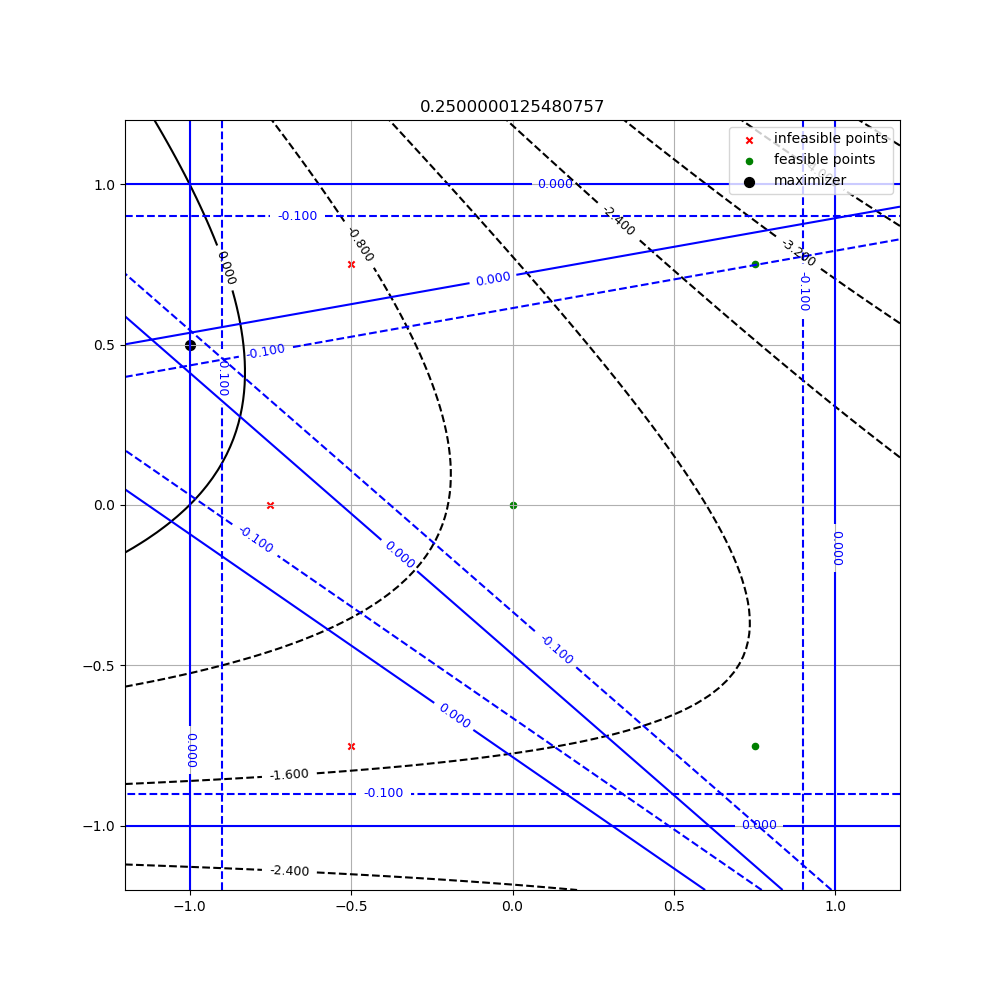
\includegraphics[width=300px]{images/pyomo_cut_solution.png}

\subsubsection{formulation}

The optimization program for finding this constraint is given by:

A set of $u^i, 1 \le i \le n_{I}$ infeasible points.
A set of $v^i, 1 \le i \le n_{F}$ feasible points.

The current Lagrange polynomial $\frac 1 2 x^T Q x + b^Tx$.
Require all infeasible point to be a distance at least $d$ from the feasible region.


Find a set of planes $(n^i, b^i), 1 \le i \le n_{P}$.

Require $n_P \ge n_I$.


What we want big:
\begin{align}
\max_{x} & \frac 1 2 x^T Q x + b^Tx &\\
 & {n^i}^T x \le b^i & \forall 1 \le i \le n_{P} \\
 & {n^i}^T v_j \le b^i & \forall 1 \le i \le n_{P}, 1\le j\le  n_{F} \\
 & {n^i}^T u_i \ge b^i + d & \forall 1 \le i \le n_{I} \\
 & \| n^i \| = 1 & \forall 1 \le i \le n_{I} \\
 & 0 \le x_i \le 1 & \forall 1 \le i \le n \\
\end{align}


A set of $v_i, 1 \le i \le n_{I}$ feasible points.




\subsection{Using a sacred region}

Another approach is to ensure that we will always have a large enough feasible region within the current trust region.

\begin{align*}
\max_{t \in \mathbb R, c \in \mathbb R^n} t \\
\| \xk - c\| \le t \\
\| {x_{inf}}_i - c \| \ge t \quad \forall i
\end{align*}

